\documentclass[tikz,border=2pt]{standalone}
\usepackage{amsmath,amssymb}
\usepackage{tikz}
\usetikzlibrary{arrows.meta}

\begin{document}
% The indicator of an event A equals 1 on A and 0 elsewhere: a Bernoulli(P(A)) variable that
% records whether A happened.
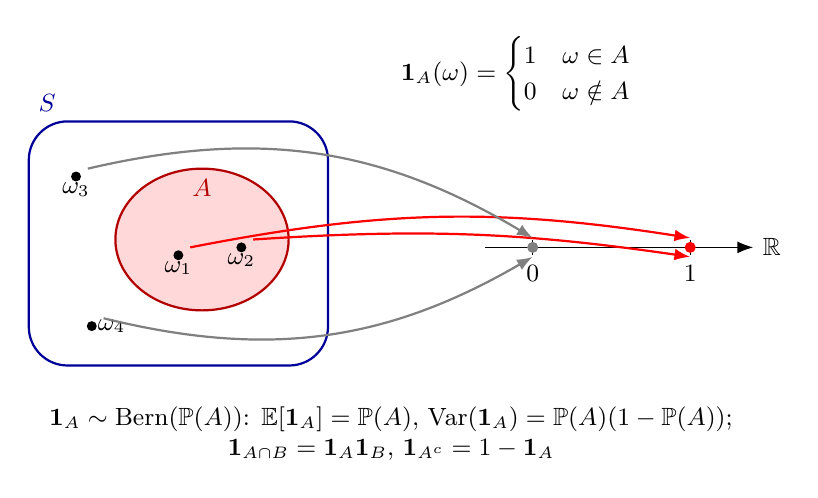
\begin{tikzpicture}[every node/.style={font=\small}, >={Latex[length=2mm]}]
	\draw[thick, blue!60!black, rounded corners=14pt] (-1.6,-1.5) rectangle (2.2,1.6);
	\node[blue!60!black, anchor=south west] at (-1.6,1.6) {$S$};
	\fill[red!15] (0.6,0.1) ellipse (1.1 and 0.9);
	\draw[red!70!black, thick] (0.6,0.1) ellipse (1.1 and 0.9);
	\node[red!70!black] at (0.6,0.75) {$A$};
	\fill (0.3,-0.1) circle (1.8pt) node[below, inner sep=2pt, font=\small] {$\omega_1$};
	\fill (1.1,0.0) circle (1.8pt) node[below, inner sep=2pt, font=\small] {$\omega_2$};
	\fill (-1.0,0.9) circle (1.8pt) node[below, inner sep=2pt, font=\small] {$\omega_3$};
	\fill (-0.8,-1.0) circle (1.8pt) node[right, inner sep=2pt, font=\small] {$\omega_4$};
	\draw[->] (4.2,0) -- (7.6,0) node[right] {$\mathbb{R}$};
	\foreach \x/\l in {4.8/0, 6.8/1} {\draw (\x,0.1) -- (\x,-0.1); \node[below=3pt] at (\x,0) {\l};}
	\draw[->, red, thick] (0.45,0.0) to[bend left=10] (6.8,0.12);
	\draw[->, red, thick] (1.25,0.1) to[bend left=6] (6.8,-0.12);
	\draw[->, gray, thick] (-0.85,1.0) to[bend left=22] (4.8,0.12);
	\draw[->, gray, thick] (-0.65,-0.9) to[bend right=22] (4.8,-0.12);
	\fill[red] (6.8,0) circle (2pt);
	\fill[gray] (4.8,0) circle (2pt);
	\node[anchor=south] at (4.6,1.6) {$\mathbf 1_A(\omega)=\begin{cases}1&\omega\in A\\0&\omega\notin A\end{cases}$};
	\node[anchor=north, align=center] at (3.0,-1.9) {$\mathbf 1_A\sim\operatorname{Bern}(\mathbb{P}(A))$: $\mathbb{E}[\mathbf 1_A]=\mathbb{P}(A)$, $\operatorname{Var}(\mathbf 1_A)=\mathbb{P}(A)(1-\mathbb{P}(A))$;\\ $\mathbf 1_{A\cap B}=\mathbf 1_A\mathbf 1_B$, $\mathbf 1_{A^c}=1-\mathbf 1_A$};
\end{tikzpicture}
\end{document}
